% AEGIS — EMNLP 2026 System Demonstrations
% Format: 6 pages max (4 content + unlimited refs), *ACL style
\documentclass[11pt]{article}
\usepackage[]{emnlp2026}
\usepackage{times,latexsym,booktabs,graphicx,hyperref,xcolor}
\usepackage{amsmath,amssymb,enumitem,microtype}
\usepackage{listings,xspace,pifont,float}

\newcommand{\system}{\textsc{Aegis}\xspace}
\newcommand{\bench}{\textsc{ToolGuard-Bench}\xspace}
\newcommand{\cmark}{{\color{green!60!black}\ding{51}}}
\newcommand{\xmark}{{\color{red!70!black}\ding{55}}}

\lstset{
  basicstyle=\scriptsize\ttfamily,
  frame=single,
  rulecolor=\color{gray!50},
  backgroundcolor=\color{gray!5},
  keywordstyle=\color{blue!70!black},
  stringstyle=\color{green!50!black},
  commentstyle=\color{gray},
  breaklines=true,
  showstringspaces=false,
  aboveskip=4pt,
  belowskip=4pt,
  xleftmargin=2pt,
  xrightmargin=2pt,
  numbers=none,
}

\title{AEGIS: No Tool Call Left Unchecked --- A Pre-Execution Firewall and Audit Layer for AI Agents}

\author{Aojie Yuan \\
  University of Southern California \\
  \texttt{aojieyua@usc.edu} \And
  Zhiyuan Su \\
  University of California, Davis \\
  \texttt{azysu@ucdavis.edu} \And
  Yue Zhao \\
  University of Southern California \\
  \texttt{yue.z@usc.edu}}

\date{}

\begin{document}
\maketitle

\begin{abstract}
Tool-using LLM agents execute database queries, shell commands, and API calls, creating a direct path from model output to real-world side effects.
We present \system, an open-source pre-execution firewall that interposes on this path with a cost-aware three-layer cascade: (L1)~pattern-based rules at sub-millisecond latency, (L2)~a supervised XGBoost classifier over 15 structural features, and (L3)~LLM-judge escalation for the few ambiguous cases.
The cascade resolves the fundamental trade-off between fast-but-brittle rules and flexible-but-expensive LLM judges. On \bench, a new benchmark of 5{,}525 tool calls from four public sources, the cascade achieves \textbf{99.9\% block rate} at \textbf{1.1\,ms median latency} and \textbf{\$0.05 total cost}---outperforming all standalone LLM judges on every metric simultaneously.
\system supports 14 agent frameworks with two-line integration, provides tamper-evident auditing via Ed25519 signatures and SHA-256 hash chains, and offers a human-in-the-loop compliance dashboard.
The system is released under MIT license.\footnote{Code: \url{https://github.com/Justin0504/Aegis}. Demo video: \url{https://www.youtube.com/watch?v=8ebpjCMRRic}}
\end{abstract}

\section{Introduction}
\label{sec:intro}

LLM agents that act through tools~\cite{yao2023react,schick2024toolformer} are moving into production, interacting with databases, file systems, and cloud infrastructure via frameworks such as LangChain~\cite{langchain2023} and CrewAI~\cite{crewai2024}.
A single hallucinated or prompt-injected tool call~\cite{greshake2023not} can cause irreversible damage before any human is aware.
Yet in most agent stacks, no enforcement layer sits between the model's tool-call decision and execution.

Post-execution observability platforms~\cite{langfuse2024,arize2024} record events after side effects occur.
Evaluation systems such as ToolEmu~\cite{ruan2024toolemu}, AgentDojo~\cite{debenedetti2024agentsec}, and InjecAgent~\cite{zhan2024injecagent} measure risk in sandboxes but do not operate on the runtime execution path.
Runtime defenses face a trade-off: rule-based layers are fast ($<$1\,ms) but miss novel attacks (0\% block rate on out-of-distribution threats in our evaluation), while LLM judges generalize well (96.6\% block) but add 1--4\,s latency and \$0.36--\$5.32 per run.

\system bridges this gap.
The key insight is that most tool calls in production are benign---cheap rules can handle them at negligible cost, while the expensive LLM judge only needs to inspect the small fraction that rules cannot resolve.
We demonstrate three novel capabilities:
\begin{enumerate}[nosep,leftmargin=*]
\item \textbf{Cost-aware cascade defense.} A three-layer pipeline (rules $\to$ XGBoost classifier $\to$ LLM judge) that short-circuits at the cheapest confident layer.
\item \textbf{Framework-agnostic interception.} Two-line integration across 14 frameworks in Python, JavaScript, and Go.
\item \textbf{Auditable enforcement.} Tamper-evident audit trails with Ed25519 signatures, human-in-the-loop approval workflows, and compliance reporting.
\end{enumerate}

\section{System Architecture}
\label{sec:arch}

Figure~\ref{fig:architecture} shows the \system architecture. The SDK layer intercepts \texttt{tool\_use} blocks from LLM API responses before execution.
Intercepted calls are forwarded to the Gateway, which runs a three-layer cascade and returns one of three decisions: \emph{allow}, \emph{block}, or \emph{pending} (routed to human review).
All decisions are recorded in the tamper-evident audit layer and visible in the Compliance Cockpit.

\begin{figure*}[t]
    \centering
    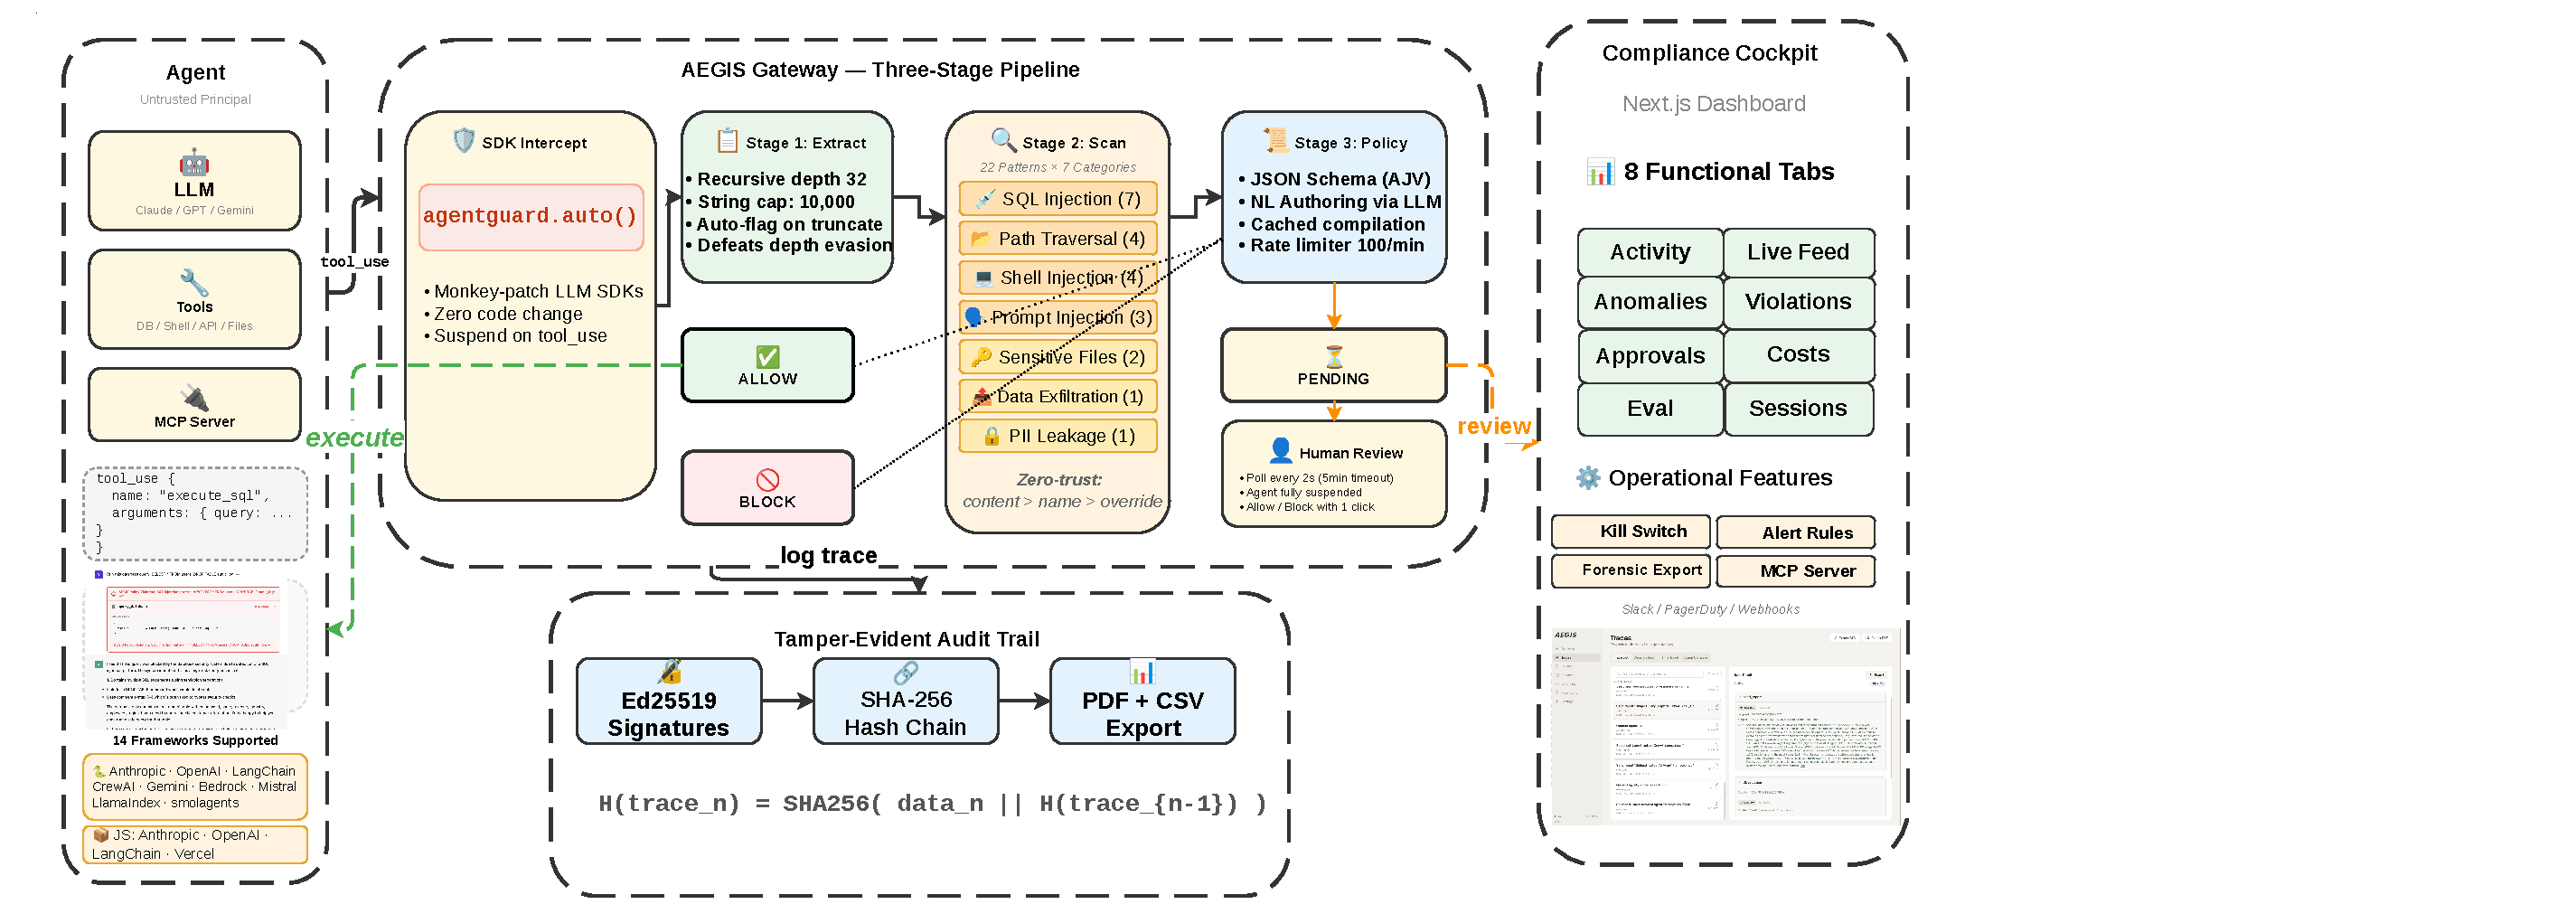
\includegraphics[width=0.93\textwidth]{figures/framework.pdf}
    \vspace{-0.1in}
    \caption{\system architecture. SDKs intercept tool calls across 14 frameworks. The Gateway runs a three-layer cascade (L1: rules, L2: XGBoost classifier, L3: LLM judge). Pending calls route to the Compliance Cockpit for human approval.}
    \vspace{-0.1in}
    \label{fig:architecture}
\end{figure*}

\subsection{SDK Layer}
\label{sec:sdk}

The SDK patches LLM client libraries at import time via \texttt{agentguard.auto()}.
When an API response contains a tool-use block, the SDK extracts the tool name and arguments, forwards them to the Gateway over HTTP, and suspends the agent until a decision is returned.
Existing agent code is unchanged:

\begin{lstlisting}[language=Python]
import agentguard
agentguard.auto()  # patches all detected SDKs
# All existing agent code runs unchanged
\end{lstlisting}

\noindent Supported frameworks: Anthropic, OpenAI, LangChain, CrewAI, Gemini, Bedrock, Mistral, LlamaIndex, smolagents~\cite{smolagents2024} (Python); Anthropic, OpenAI, LangChain, Vercel AI SDK (JS/TS); and Go.

\subsection{Three-Layer Cascade}
\label{sec:cascade}

The cascade is the core enforcement mechanism:

\paragraph{L1: Pattern-Based Rules ($<$1\,ms).}
22 detection patterns across 7 categories---SQL injection (7 patterns), path traversal (4), shell injection (4), prompt injection (3), sensitive file access (2), data exfiltration (1), PII leakage (1)---are matched against recursively extracted argument strings (depth limit 32). If a pattern fires, the call is immediately blocked.

\paragraph{L2: Supervised Behavioral Classifier ($<$10\,ms).}
Each tool call is encoded into a 15-dimensional feature vector (Table~\ref{tab:features}) capturing argument structure (count, depth, length), character-level statistics (digit/uppercase/punctuation ratios, Shannon entropy), and content indicators (URL count, IP literals, path separators, base64/hex-like scores).
A gradient-boosted tree classifier (XGBoost, 300 trees, depth~6) outputs $P(\text{malicious}) \in [0,1]$.
Two calibrated thresholds control the cascade: calls below $\tau_l$ (confident benign) are allowed; calls above $\tau_h$ (confident malicious) are blocked; ambiguous calls in $[\tau_l, \tau_h]$ escalate to L3.
The L2 backend is pluggable: we also evaluate an unsupervised Isolation Forest~\cite{zhao2019pyod} for deployments without labeled data.

\begin{table}[t]
\centering
\scriptsize
\caption{L2 feature vector (15 dims). All features are extracted from tool arguments in $<$10\,ms without any LLM call.}
\vspace{-0.1in}
\label{tab:features}
\setlength{\tabcolsep}{2.5pt}
\begin{tabular}{rll}
\toprule
\# & Feature & Description \\
\midrule
1--3 & arg\_count, total\_chars, depth & Structure \\
4--5 & url\_count, ip\_literals & Network indicators \\
6--8 & digit/upper/punct\_ratio & Character distribution \\
9--11 & json\_depth, path\_sep, braces & Format signals \\
12 & shannon\_entropy & Randomness (bits/char) \\
13--15 & longest\_run, base64, hex & Encoding heuristics \\
\bottomrule
\end{tabular}
\vspace{-0.15in}
\end{table}

\paragraph{L3: LLM Judge ($\sim$1--2\,s).}
A zero-shot prompt to a frontier model (e.g., Claude Haiku~4.5) classifies the tool call as malicious or benign.
Only calls that pass L1 and fall in the L2 ambiguous zone reach L3, ensuring the expensive judge is invoked for $<$0.3\% of production calls.

\paragraph{Short-Circuit Logic.}
$\text{L1}_\text{block} \to \text{block}$; else $\text{L2} < \tau_l \to \text{allow}$; else $\text{L2} \ge \tau_l \to \text{escalate to L3}$.
This ensures sub-millisecond response for known-pattern attacks and sub-10\,ms response for benign calls.

\subsection{Audit Layer and Compliance Cockpit}
\label{sec:audit}

Each trace is signed with a per-agent Ed25519 key~\cite{bernstein2012eddsa} and linked into a SHA-256 hash chain.
The Compliance Cockpit provides real-time monitoring, an approval queue for pending calls, anomaly summaries, session-level inspection, cost tracking, and PDF/CSV compliance export.

\section{Evaluation}
\label{sec:eval}

We validate \system on \bench, a benchmark we release alongside the system.

\paragraph{Benchmark.}
\bench contains 5{,}525 tool calls (3{,}413 malicious, 2{,}112 benign) from four public sources (Table~\ref{tab:bench}).
Each record is tagged with a distribution-shift label relative to AEGIS rules: \emph{in-distribution} (crafted to match L1), \emph{near-OOD} (InjecAgent prompt-injection attacks), and \emph{far-OOD} (OWASP payloads).

\input{figures/table_1_benchmark}

\paragraph{Baselines.}
We compare 10 configurations: four LLM judges (GPT-4o-mini, GPT-4o, Claude Haiku~4.5, Claude Sonnet~4.6), Llama-Guard-3-8B on GPU, keyword blacklist, AEGIS-rules (L1 only), AEGIS-L2 only, the full AEGIS cascade (L1+L2+L3), and no defense.

\paragraph{Main Results.}
Table~\ref{tab:overall} shows headline metrics.
With XGBoost L2, the AEGIS cascade achieves \textbf{99.9\% block rate} with 0.09\% FP at \textbf{1.1\,ms} median latency and \textbf{\$0.05} total cost---outperforming every standalone LLM judge on all four metrics simultaneously.
Even the best LLM judge (GPT-4o-mini, 98.8\% block) has 11.88\% false positives and 1{,}204\,ms latency.
The unsupervised IForest variant achieves 94.1\% block rate with 0\% FP but at 2{,}146\,ms and \$4.18, showing the value of supervised L2.

\input{figures/table_3_overall}

\paragraph{Generalization.}
Table~\ref{tab:perdist} reveals the cascade's value: L1 rules achieve 77.4\% on in-distribution attacks but \textbf{0\%} on near-OOD InjecAgent attacks.
The LLM judge (Haiku) improves from 77.4\% in-dist to 96.9\% near-OOD, demonstrating semantic generalization.
The cascade captures this via L3 escalation: 79.2\% in-dist, 94.3\% near-OOD, 100\% far-OOD.

\input{figures/table_2_per_distribution}

\paragraph{Per-Layer Resolution and L2 Ablation.}
With supervised XGBoost L2, the cascade resolves 96.3\% of calls at L2 ($<$1\,ms), with only 1.6\% reaching the expensive L3 LLM judge---a 46$\times$ reduction versus the unsupervised IForest variant (92.7\% reaching L3).
L2 alone (XGBoost, no L3) achieves 99.8\% block rate at 0.82\,ms P50, confirming the classifier's discriminative power.
The unsupervised IForest L2 alone achieves only 0.67\% block rate, showing that supervised training is essential for L2 to carry the cascade's detection burden.

\paragraph{Production Cost.}
The XGBoost cascade costs \$0.05 per full benchmark run (5{,}525 calls), compared to \$0.36--\$5.32 for standalone LLM judges.
In realistic traffic ($\ge$99\% benign), the effective per-call cost drops below \$0.00001.

\paragraph{Cross-Source Generalization.}
To test for same-source bias, we evaluate XGBoost L2 in cross-source settings (Table~\ref{tab:xsource}).
Training on InjecAgent and testing on ToolEmu+OWASP yields only 27.2\% block rate, confirming that the classifier learns source-specific patterns.
Training on ToolEmu+OWASP and testing on InjecAgent yields 89.4\%.
This motivates the cascade design: L2 handles calls that match training distribution at $<$3\,ms, while L3 (LLM judge) catches the OOD remainder---combining speed with generalization.

\begin{table}[t]
\centering\small
\caption{Cross-source generalization of XGBoost L2 (no L3). Block rate drops on OOD sources, validating the need for L3 as a generalization backstop.}
\vspace{-0.1in}
\label{tab:xsource}
\begin{tabular}{llrr}
\toprule
Train source & Test source & Block\% & FP\% \\
\midrule
InjecAgent & InjecAgent (held-out) & 93.4 & 0.00 \\
InjecAgent & ToolEmu+OWASP+Self & 27.2 & 0.00 \\
ToolEmu+OWASP+Self & InjecAgent & 89.4 & 0.00 \\
\bottomrule
\end{tabular}
\vspace{-0.1in}
\end{table}

\paragraph{Adaptive Robustness.}
An LLM-driven red-team attacker (Sonnet~4.6) iteratively rewrites 53 malicious seeds over 5 rounds.
The keyword blacklist is bypassed 52.8\% of the time; AEGIS rules at 17.0\%; the LLM judge at 11.3\%.
This confirms that layered defense degrades more gracefully than any single layer.

\input{figures/table_5_adaptive}

\section{Demonstration}
\label{sec:demo}

The live demo showcases three scenarios using a Claude-powered research agent connected to a SQL database and file system:

\begin{enumerate}[nosep,leftmargin=*]
\item \textbf{Benign workflow.}
A user asks ``\emph{Summarize feedback from the reviews table.}''
The agent generates a \texttt{SELECT} query; \system classifies it as LOW risk via L1 in $<$1\,ms and allows execution.
The Compliance Cockpit shows the trace in real time.

\item \textbf{Attack interception.}
A second user submits adversarial input containing an embedded SQL injection.
The agent produces a destructive query; \system blocks it at L1 in 6.2\,ms.
The agent receives a block decision and gracefully informs the user.
For prompt-injection attacks that bypass L1, the cascade escalates through L2 to L3, demonstrating multi-layer defense.

\item \textbf{Human-in-the-loop approval.}
A high-risk shell command (\texttt{kubectl delete pod}) triggers a \texttt{pending} decision.
The agent pauses. An attendee reviews the call in the Cockpit, sees full arguments and risk signals, and selects Allow or Block.
The agent resumes within one polling cycle.
\end{enumerate}

\noindent Attendees can submit their own adversarial inputs during the demo and observe the cascade's layer-by-layer response in the Cockpit.

\section{Related Work}
\label{sec:related}

\paragraph{Agent Safety Benchmarks.}
ToolEmu~\cite{ruan2024toolemu} emulates tool execution for LLM-based risk scoring; AgentDojo~\cite{debenedetti2024agentsec} studies prompt injection in dynamic environments; InjecAgent~\cite{zhan2024injecagent} benchmarks indirect prompt injection.
These systems evaluate risk in sandboxes.
\system enforces pre-execution control on live tool calls and uses these benchmarks for out-of-distribution validation.

\paragraph{LLM Trustworthiness.}
TrustLLM~\cite{huang2024position} and TrustEval~\cite{wang2024trusteval} assess trustworthiness at the model level.
\system operates at the \emph{action} level, enforcing trust boundaries on tool calls.

\paragraph{Observability Platforms.}
Langfuse~\cite{langfuse2024}, Helicone~\cite{helicone2024}, and Arize~\cite{arize2024} provide post-execution tracing.
\system complements these by mediating calls before side effects occur.

\paragraph{LLM Guardrails.}
Llama Guard~\cite{inan2023llama} and NeMo Guardrails classify text safety.
\system differs in scope: it inspects structured tool calls (not free-form text), applies a cost-aware cascade to minimize latency, and integrates human approval and cryptographic auditing.

\section{Conclusion}

We presented \system, a pre-execution firewall for tool-using LLM agents.
The cost-aware cascade resolves the trade-off between cheap rules and expensive LLM judges: with a supervised XGBoost L2 classifier, the cascade achieves 99.9\% block rate at 1.1\,ms median latency and \$0.05 total cost---outperforming all standalone LLM judges on every metric.
The system supports 14 frameworks, provides tamper-evident auditing, and is open-source.

\bibliography{references}
\bibliographystyle{acl_natbib}

\end{document}
